\section{Projeto de Pontes de Madeira}\label{sec:ponte_madeira}

Esta seção apresenta os critérios de dimensionamento adotados para pontes de madeira em viga de toras roliças, compreendendo as ações do trem tipo, os ponderadores das propriedades mecânicas, os limites de flecha e o roteiro de verificação da longarina e do tabuleiro.

\subsection{Carga do trem tipo}\label{sec:trem_tipo}

As cargas móveis das pontes rodoviárias brasileiras são definidas pela \textcite{nbr7188} em seu item 5.1.1. Por se tratar de estradas vicinais, adota-se o TB-240, caracterizado por um veículo de 240 kN de peso total, constituído por seis rodas e três eixos, com carga de 40 kN por roda e espaçamentos de 1,5 m entre os eixos.
A área de ocupação do veículo deve ser de 18,0 m², complementada por uma carga
uniformemente distribuída de 4,0 kN/m² em seu entorno (multidão), conforme a Figura \ref{fig:trem}.

\begin{figure}[htpb!]
\centering
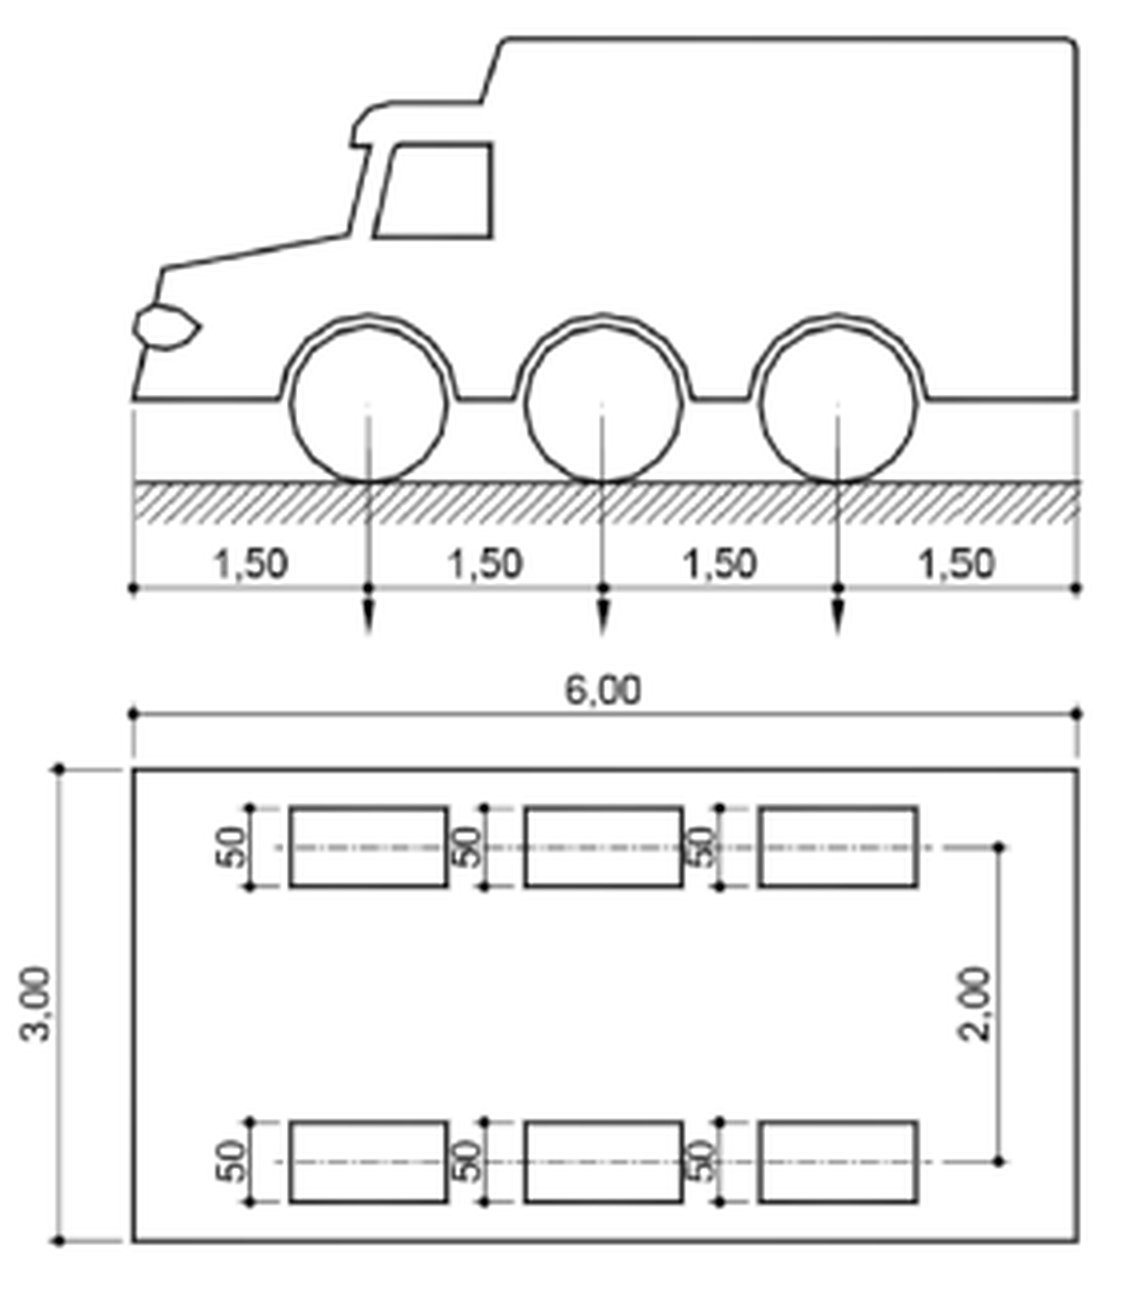
\includegraphics[width=0.4\textwidth]{figuras/trem1_hq.png}
\caption{Configuração trem de tipo \parencite{nbr7188}.}
\label{fig:trem}
\end{figure}

\subsection{Ponderadores para propriedades mecânicas}

Para as verificações estruturais, a \textcite{NBR7190-1:2022} estabelece parâmetros de resistência ($f$) e de módulo de elasticidade ($E$), bem como classes de resistência para madeiras dos grupos das Coníferas e das Folhosas, sob condição padrão de referência, isto é, teor de umidade ($U$) igual a 12\%.

O método dos estados limites baseia-se na premissa de majoração dos esforços e minoração das resistências ($f$) e do módulo de elasticidade ($E$).
Os coeficientes de minoração têm por objetivo compensar as incertezas associadas à resistência característica, bem como os efeitos adversos das imperfeições geométricas.
A \textcite{NBR7190-1:2022} propõe essa minoração por meio da utilização dos coeficientes de modificação ($k_{\mathrm{mod}}$) e do coeficiente de ponderação da resistência ($\gamma_w$), conforme apresentado na Equação~\eqref{eq:2.099}.

\begin{equation}
    X_d = \frac{k_{\mathrm{mod}} \cdot X_k}{\gamma_w}
\label{eq:2.099}
\end{equation}
Onde:
\begin{itemize}
    \item $X_k$ é o valor característico da resistência da madeira;
    \item $k_{\mathrm{mod}}$ é o coeficiente de modificação da madeira;
    \item o coeficiente de ponderação da resistência ($\gamma_w$) assume o valor de 1{,}4 para tensões normais e 1{,}8 para tensões de cisalhamento.
\end{itemize}

O coeficiente de modificação ($k_{\mathrm{mod}}$) altera os valores característicos das propriedades de resistência da madeira em função da classe de carregamento da estrutura e da classe de umidade admitida, sendo calculado conforme a Equação~\eqref{eq:2.99}.

\begin{equation}
k_{\mathrm{mod}} = k_{\mathrm{mod},1} \cdot k_{\mathrm{mod},2}
\label{eq:2.99}
\end{equation}

O primeiro fator, $k_{\mathrm{mod},1}$, está associado à classe de carregamento, sendo definido em função da duração acumulada da ação variável principal da combinação e do tipo de madeira empregado, de acordo com o item 5.8.4.1 da \textcite{NBR7190-1:2022}. Os valores correspondentes às diferentes classes de carregamento e aos grupos de materiais são apresentados na Tabela \ref{tab:kmod1.q}.

\begin{table}[htpb!]
\centering
\caption{Classes de carregamento e fatores de modificação (\textit{$k_{mod,1}$}) \parencite{NBR7190-1:2022}.}
\label{tab:kmod1.q}
\footnotesize
\begin{tabular}{
>{\centering\arraybackslash}m{2.8cm}
>{\centering\arraybackslash}m{2.2cm}
>{\centering\arraybackslash}m{3.8cm}
>{\centering\arraybackslash}m{4.6cm}
>{\centering\arraybackslash}m{1.8cm}
}
\hline
\multirow{4}{*}{\shortstack{\textbf{Classes de} \\ \textbf{carregamento}}} &
\multicolumn{2}{c}{\textbf{Ação variável principal da combinação}} &
\multirow{4}{*}{\shortstack{\textbf{Tipos de} \\ \textbf{madeira}\textsuperscript{a}}} &
\multirow{4}{*}{\shortstack{\textbf{Madeira} \\ \textbf{Recomposta}}}\\
\cline{2-3}
& \textbf{Duração acumulada} &
\textbf{Ordem de grandeza da duração acumulada da ação característica} &
& \\
\hline
Permanente &
Permanente &
Mais de dez anos &
0,60 &
0,30 \\
%\hline
Longa duração &
Longa duração &
Seis meses a dez anos &
0,70 &
0,45 \\
%\hline
Média duração &
Média duração &
Uma semana a seis meses &
0,80 &
0,65 \\
%\hline
Curta duração &
Curta duração &
Menos de uma semana &
0,90 &
0,90 \\
%\hline
Instantânea &
Instantânea &
Muito curta &
1,10 &
1,10 \\
\hline
\end{tabular}

\vspace{0.2cm}
\centering
\footnotesize\textsuperscript{a}\,Madeira serrada, madeira roliça, madeira laminada colada (MLC), madeira laminada colada cruzada (MLCC) e madeira laminada colada de lâminas paralelas (LVL).
\end{table}

A \textcite{NBR7190-1:2022} não classifica explicitamente a ação do tráfego rodoviário quanto à sua duração acumulada.
O item 2.3.1.2 do \textcite{EN1995-2:2004} e o item NA.2.1 do Anexo Nacional britânico \textcite{BSNA-EN1995-2:2004} classificam as ações variáveis decorrentes da passagem de veículos e de pedestres como ações de \emph{curta duração} (\textit{short-term actions}), em razão de seu caráter transitório e não sustentado, distinto das ações permanentes ou de longa duração que dominam a Tabela \ref{tab:kmod1.q}. 

A classe de umidade adotada permanece a (3), compatível com elementos estruturais expostos ao tempo, mas protegidos do contato direto com a água, condição típica das pontes de madeira roliça em estradas vicinais.

O segundo fator, $k_{\mathrm{mod},2}$, está relacionado à classe de umidade à qual o elemento estrutural está submetido, bem como ao tipo de material utilizado, conforme especificado no item 5.8.4.2 da \textcite{NBR7190-1:2022}.
Os valores normativos desse coeficiente, diferenciados entre madeiras maciças, produtos engenheirados e madeiras recompostas, encontram-se sistematizados na Tabela \ref{tab:kmod2.2}.

\begin{table}[htpb!]
\centering
\caption{Valores de (\textit{$k_{mod,2}$}) \parencite{NBR7190-1:2022}.}
\label{tab:kmod2.2}
\footnotesize
\begin{tabular}{
>{\centering\arraybackslash}p{3cm}
>{\centering\arraybackslash}p{6cm}
>{\centering\arraybackslash}p{2cm}
}
\hline
\multirow{2}{*}{\textbf{Classes de umidade}} &
\multirow{2}{*}{\textbf{Tipos de madeira}} &
\textbf{Madeira recomposta} \\
\hline
 &  Madeira serrada \newline
Madeira roliça \newline
Madeira laminada colada (MLC) \newline
Madeira laminada colada cruzada (MLCC) \newline
Madeira laminada colada (LVL) & \\
\hline
(1) & 1,00 & 1,00 \\
%\hline
(2) & 0,90 & 0,95 \\
%\hline
(3) & 0,80 & 0,93 \\
%\hline
(4) & 0,70\textsuperscript{a} & 0,90 \\
\hline
\end{tabular}

\vspace{0.2cm}
\centering
\footnotesize\textsuperscript{a}\,Não é permitido o uso do MLCC para classe de umidade (4).
\end{table}

\subsection{Flecha limite}\label{sec:flecha_limite}

\subsubsection{Fluência}

As flechas instantâneas, $\delta_{\mathrm{inst},G_i,k}$ e $\delta_{\mathrm{inst},Q_j,k}$, associadas respectivamente às ações permanentes e variáveis, são calculadas com o módulo de elasticidade médio à flexão, $E_{0,\mathrm{m}}$. O efeito do tempo sobre a rigidez é incorporado separadamente, por meio do coeficiente de fluência $\varphi$, que amplia as flechas instantâneas para obter as flechas finais $\delta_{\mathrm{fin},G_i,k}$ e $\delta_{\mathrm{fin},Q_j,k}$, conforme as Equações~\eqref{eq:flecha_fin_G} e~\eqref{eq:flecha_fin_Q}.

\begin{equation}
\delta_{\mathrm{fin},G_i,k}
=
\delta_{\mathrm{inst},G_i,k}
+ \delta_{\mathrm{creep}}
=
\delta_{\mathrm{inst},G_i,k} \cdot (1 + \varphi)
\label{eq:flecha_fin_G}
\end{equation}

\begin{equation}
\delta_{\mathrm{fin},Q_j,k}
=
\delta_{\mathrm{inst},Q_j,k}
+ \delta_{\mathrm{creep}}
=
\delta_{\mathrm{inst},Q_j,k} \cdot \psi_{2} \cdot (1 + \varphi)
\label{eq:flecha_fin_Q}
\end{equation}

Segundo a \textcite{NBR7190-1:2022}, ``a madeira possui características distintas de outros materiais de construção, como, por exemplo, a significativa deformação ao longo do tempo (fluência)''.
Em razão dessa condição, torna-se necessária a aplicação do coeficiente de fluência ($\varphi$) na estimativa dos deslocamentos finais ou efetivos, conforme as Equações~\eqref{eq:flecha_fin_G} e~\eqref{eq:flecha_fin_Q}.
Esse coeficiente é definido em função do material e da classe de umidade à qual o sistema estrutural está exposto.
Classes de umidade mais elevadas resultam em flechas mais acentuadas, conforme evidenciado pelos valores do coeficiente de fluência da \ref{tab:fluencia}.

\begin{table}[htpb!]
\centering
\caption{Coeficiente de fluência ($\varphi$). Adaptado do item 8.1 tabela 20 da \textcite{NBR7190-1:2022}.}
\label{tab:fluencia}
\footnotesize
\begin{tabular}{
>{\centering\arraybackslash}m{6.0cm}
>{\centering\arraybackslash}m{2.5cm}
>{\centering\arraybackslash}m{2.5cm}
>{\centering\arraybackslash}m{2.5cm}
}
\hline
\multirow{2}{*}{\textbf{Materiais}} &
\multicolumn{3}{c}{\textbf{Classe de umidade}} \\
\cline{2-4}
& \textbf{(1)} & \textbf{(2 e 3)} & \textbf{(4)} \\
\hline
Madeira serrada, MLC, MLCC, LVL e roliça
& 0,6 & 0,8 & 2,0\textsuperscript{a} \\
\hline
Compensado estrutural
& 0,8 & 1,0 & 2,5 \\
\hline
OSB estrutural
& 1,5 & 2,25 & -- \\
\hline
\end{tabular}

\vspace{0.3cm}
\small\textsuperscript{a} Não é permitido o uso de MLCC para a classe de umidade 4.
\end{table}

Para a classe de umidade (3) adotada neste trabalho, o coeficiente de fluência de referência é $\varphi = 0{,}8$.

\subsubsection{Limites normativos de flecha}

Na verificação do Estado Limite de Serviço (ELS), o item 8.2 da \textcite{NBR7190-1:2022} estabelece valores limites para as flechas, considerando-se a flecha instantânea ($\delta_{\mathrm{inst}}$) e a flecha final ($\delta_{\mathrm{fin}}$).
Esses valores limites dependem da configuração estática da estrutura e encontram-se apresentados na Tabela \ref{tab:flechas_limites}.

\begin{table}[htpb!]
\centering
\caption{Flechas limites para elementos correntes fletidos \parencite{NBR7190-1:2022}.}
\label{tab:flechas_limites}
\footnotesize
\begin{tabular}{
>{\centering\arraybackslash}m{5.0cm}
>{\centering\arraybackslash}m{3.0cm}
>{\centering\arraybackslash}m{3.0cm}
}
\hline
\textbf{Tipo} & $\boldsymbol{\delta_{inst}}$ & $\boldsymbol{\delta_{fin}}$ \\
\hline
Vigas biapoiadas ou contínuas
& L/300 a L/500
& L/150 a L/300 \\
\hline
Vigas em balanço
& L/150 a L/250
& L/75 a L/150 \\
\hline
\end{tabular}

\end{table}

Logo, o dimensionamento de sistemas estruturais em madeira deve atender a esses requisitos normativos.

\subsection{Projeto da ponte}\label{sec:projeto_ponte}

O sistema estrutural considerado é composto por um tabuleiro de pranchas retangulares de madeira, de largura $b_w$ e altura $h$, apoiado continuamente sobre longarinas circulares roliças de diâmetro $d$, tratadas analiticamente como vigas biapoiadas de vão $L$.
As etapas de verificação seguem a sequência: determinação dos esforços solicitantes, verificação à flexão e ao cisalhamento da longarina, verificação da flecha e, por fim, verificação à flexão do tabuleiro.
O procedimento de cálculo apresentado nesta seção segue os critérios normativos da \textcite{NBR7190-1:2022} e o roteiro de dimensionamento do Manual de Projeto e Construção de Pontes de Madeira de \textcite{CALIL2006}.

\subsubsection{Esforços}

Para a longarina circular maciça, a área, o momento de inércia, o módulo resistente e o raio de giração são obtidos pelas Equações~\eqref{eq:areacirc} a~\eqref{eq:rcirc}.

\begin{equation}
A = \frac{\pi d^2}{4}
\label{eq:areacirc}
\end{equation}

\begin{equation}
I_x = I_y = \frac{\pi d^4}{64}
\label{eq:icirc}
\end{equation}

\begin{equation}
W_x = W_y = \frac{I_x}{d/2}
\label{eq:wcirc}
\end{equation}

\begin{equation}
r_x = r_y = \sqrt{\frac{I_x}{A}}
\label{eq:rcirc}
\end{equation}

Para as pranchas retangulares do tabuleiro, a área e o momento de inércia em relação ao eixo de flexão são dados pelas Equações~\eqref{eq:arearet} e~\eqref{eq:iret}.

\begin{equation}
A = b_w\,h
\label{eq:arearet}
\end{equation}

\begin{equation}
I_x = \frac{b_w\,h^3}{12}
\label{eq:iret}
\end{equation}

As ações permanentes correspondem ao peso próprio das longarinas, do tabuleiro e demais elementos, obtidas em função da geometria e do peso específico $\gamma$, conforme a Equação~\eqref{eq:permanente}.

\begin{equation}
G = \gamma \cdot A
\label{eq:permanente}
\end{equation}

A carga móvel considerada é o trem-tipo TB-240 apresentado na Seção~\ref{sec:trem_tipo}, representado por um veículo de três eixos e seis rodas, cada roda transmitindo uma carga $P$ de 40~kN, além da carga de multidão, uniformemente distribuída na área de ocupação com o valor característico $q_A = 4{,}0$~kN/m\textsuperscript{2}.
Como as longarinas são tratadas como vigas isoladas, a carga de multidão precisa ser convertida de carga de área em carga linear antes de entrar nas Equações~\eqref{eq:mqk45} e~\eqref{eq:qqk}, multiplicando-se $q_A$ pela largura tributária de cada longarina, isto é, pelo espaçamento corrigido entre longarinas $esp_{long,corr}$ (Seção~\ref{sec:formulacao}), conforme a Equação~\eqref{eq:qlong}.

\begin{equation}
q = q_A \cdot esp_{long,corr}
\label{eq:qlong}
\end{equation}

O espaçamento corrigido entre longarinas $esp_{long,corr}$ corresponde a dimensão geométrica inteira que o otimizador usa em todo o seu processo de cálculo de restrições e cálculo da função objetivo. Como a otimização será tratada como continua esse valor precisa ser revisado para "dimensões comerciais" inteiras.

Os efeitos dinâmicos são incorporados pelo coeficiente de impacto vertical ($CIV$), determinado pelas Equações~\eqref{eq:civ1} e~\eqref{eq:civ2} conforme o item 5.1.3.1 da \textcite{nbr7188}, sendo $LIV$ o comprimento característico da estrutura.

\begin{equation}
CIV = 1{,}35 \qquad \text{para } L \leq 10{,}0\ \text{m}
\label{eq:civ1}
\end{equation}

\begin{equation}
CIV = 1 + 1{,}06\left(\frac{20}{LIV + 50}\right), \qquad \text{para } 10{,}0 < L \leq 200{,}0\ \text{m}
\label{eq:civ2}
\end{equation}

O $CIV$ multiplica diretamente os esforços solicitantes de origem variável.

O momento fletor e o esforço cortante máximos devidos à carga permanente, assim como a flecha estática correspondente, são quantificados pelas premissas clássicas de estática para vigas biapoiadas, conforme as Equações~\eqref{eq:mgk} e~\eqref{eq:qgk}.

\begin{equation}
M_{gk} = \frac{g\,L^2}{8}
\label{eq:mgk}
\end{equation}

\begin{equation}
Q_{gk} = \frac{g\,L}{2}
\label{eq:qgk}
\end{equation}

Os efeitos do trem tipo são empregados usados conceitos de análise de estruturas e a as recomendações de \textcite{CALIL2006}.

\subsubsection*{Momento fletor e flecha}

Para o momento fletor e para a flecha, o veículo é centralizado no vão: a roda central posiciona-se exatamente no meio do vão, com as duas rodas externas a uma distância $a$ dela, conforme a Figura~\ref{fig:posicao_momento_flecha}.

\begin{figure}[!ht]
    \centering
    \begin{subfigure}{0.75\textwidth}
        \centering
        
\includegraphics[width=\textwidth]{figuras/posicionamento_momento_flecha.png}
        \caption{Momento fletor e flecha.}
        \label{fig:posicao_momento_flecha}
    \end{subfigure}

    \vspace{0.2cm}
    \begin{subfigure}{0.75\textwidth}
        \centering
        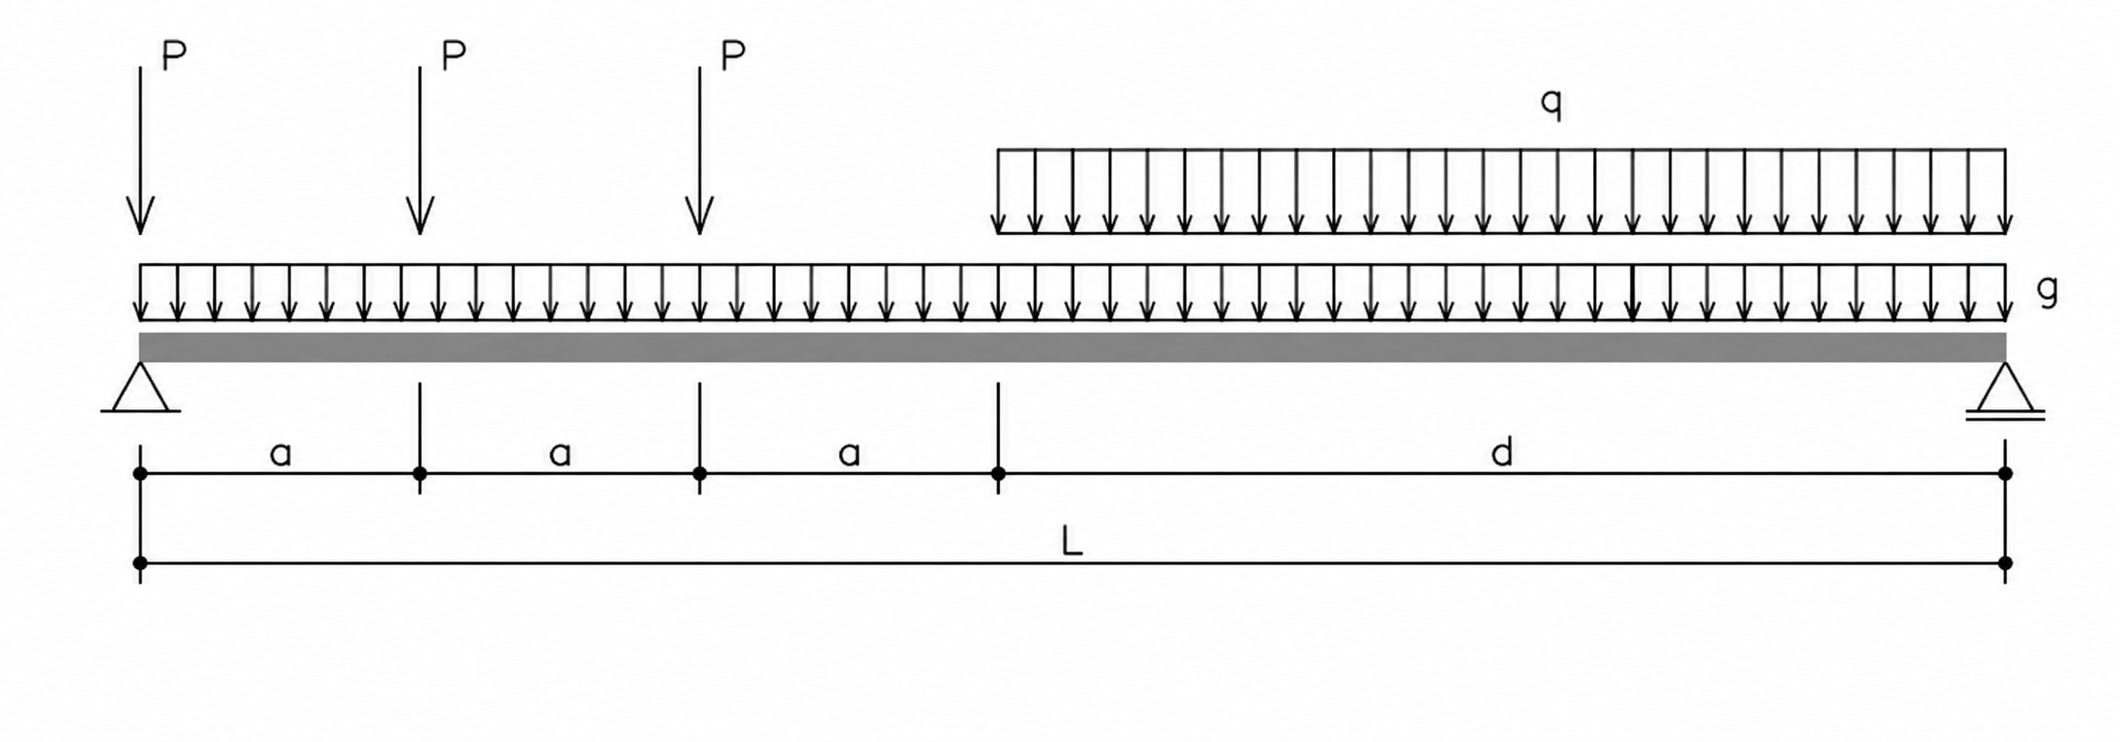
\includegraphics[width=\textwidth]{figuras/posicionamento_reacao_apoio.png}
        \caption{Reação de apoio.}
        \label{fig:posicao_reacao}
    \end{subfigure}

    \vspace{0.2cm}
    \begin{subfigure}{0.75\textwidth}
        \centering
        
\includegraphics[width=\textwidth]{figuras/posicionamento_cortante.png}
        \caption{Esforço cortante.}
        \label{fig:posicao_cortante}
    \end{subfigure}
    \caption{Posicionamento do veículo-tipo para o cálculo dos esforços na longarina \parencite{CALIL2006}.}
    \label{fig:posicionamentos}
\end{figure}

O momento fletor máximo sob a roda central resulta da Equação~\eqref{eq:mqk30}, escrita para $3\,\text{m} < L \leq 6\,\text{m}$. Já para vãos maiores que 6 metros a~Equação~\eqref{eq:mqk45} representa o esforço máximo.

\begin{equation}
c = \frac{L - 4a}{2}, \qquad \text{para } L > 6\,\text{m}
\label{eq:cmomento}
\end{equation}

\begin{equation}
M_{qk} = \frac{3\,P\,L}{4} - P\,a, \qquad \text{para } 3\,\text{m} < L \leq 6\,\text{m}
\label{eq:mqk30}
\end{equation}

\begin{equation}
M_{qk} = \left(\frac{3\,P\,L}{4} - P\,a\right) + \frac{q\,c^2}{2}, \qquad \text{para } L > 6\,\text{m}
\label{eq:mqk45}
\end{equation}

A posição centralizada, contudo, só é a posição de máximo esforço enquanto as três rodas permanecem efetivamente carregando o vão. Com as rodas externas a $L/2 \pm a$ do apoio esquerdo, elas alcançam os apoios quando $L = 2a$; a partir daí passam a ter braço nulo, ou a sair do vão, e o arranjo centralizado deixa de maximizar o momento. Para $a = 1{,}5$~m e $L = 3{,}0$~m, as rodas externas assentam exatamente sobre os apoios e a Equação~\eqref{eq:mqk30} degenera no caso de carga única centrada, $M_{qk} = PL/4$.

Nesse caso, o momento máximo é encontrado posicionando o trem-tipo de forma que apenas duas rodas fiquem dentro do vão, seguindo o Teorema de Barré: o centro do vão deve ficar exatamente no ponto médio entre uma das cargas e a resultante do par. Essa condição leva à posição $x = (2L-a)/4$ para a primeira roda, e o momento máximo é dado pela Equação~\eqref{eq:mqk2}, obtida maximizando $M(x) = P\,x\,(2L - 2x - a)/L$.

\begin{equation}
M_{qk}^{(2)} = \frac{P\,(2L-a)^2}{8L}, \qquad \text{válida para } L \geq 1{,}5\,a
\label{eq:mqk2}
\end{equation}

A envoltória do momento devido à carga móvel é, portanto, o maior valor entre os arranjos admissíveis, conforme a Equação~\eqref{eq:mqkenv}: três rodas centralizadas, duas rodas na posição de Barré, ou uma única roda no meio do vão.

\begin{equation}
M_{qk} = \max\left(\frac{3PL}{4} - Pa\;,\;\; \frac{P\,(2L-a)^2}{8L}\;,\;\; \frac{PL}{4}\right)
\label{eq:mqkenv}
\end{equation}

O primeiro termo domina para $L \geq 2{,}23\,a$, isto é, $L \geq 3{,}34$~m quando $a = 1{,}5$~m, de modo que a Equação~\eqref{eq:mqkenv} recupera a Equação~\eqref{eq:mqk30} em toda a faixa usual e dela difere apenas nos vãos mais curtos: no vão de $3{,}0$~m, a formulação centralizada fornece $30{,}0$~kN$\cdot$m contra $33{,}75$~kN$\cdot$m da envoltória, uma subestimativa de $12{,}5\%$. Para $L > 6$~m, em que a parcela de multidão passa a existir, o arranjo centralizado domina com ampla margem e a Equação~\eqref{eq:mqk45} permanece governando.

A mesma posição centralizada da Figura~\ref{fig:posicao_momento_flecha} é usada para a flecha (Seção~\ref{sec:formulacao}, Equações~\eqref{eq:flechag} e~\eqref{eq:flechaq}), com $b$ a distância entre o apoio e a roda externa mais próxima.

\subsubsection*{Reação de apoio}

Para a reação de apoio, o veículo é posicionado encostado no apoio de interesse, conforme a Figura~\ref{fig:posicao_reacao}, e não centralizado como no caso do momento: aproximar o grupo de cargas do apoio maximiza a parcela de cada roda que se transfere diretamente para ele.

\subsubsection*{Esforço cortante}

Para o cortante, a Figura~\ref{fig:posicao_cortante} mostra o veículo afastado do apoio por $2h$, sendo $h$ a altura (ou o diâmetro, para seção circular) da peça: a \textcite{NBR7190-1:2022} permite avaliar o cortante em uma seção afastada do apoio, e não na face do apoio propriamente dita.
Essa posição fornece a grandeza auxiliar $e$ da Equação~\eqref{eq:ecortante} e o cortante de cálculo $Q_{qk}$ da Equação~\eqref{eq:qqk}.

\begin{equation}
e = L - 3a - 2h
\label{eq:ecortante}
\end{equation}

\begin{equation}
Q_{qk} = \frac{P}{L}\,(6a + 3e) + \frac{q\,e^2}{2\,L}
\label{eq:qqk}
\end{equation}

A Equação~\eqref{eq:qqk} pressupõe, contudo, que todo o esquema de carregamento caiba no vão: afastado o veículo por $2h$ do apoio, ainda precisa sobrar comprimento para as três rodas e para a parcela de multidão, isto é, $L \geq 2h + 3a$. Essa condição é folgada em vigas usuais, mas deixa de valer justamente na faixa de interesse deste trabalho, em que o diâmetro da longarina roliça não é desprezível frente ao vão. Quando $e$ resulta negativo, a Equação~\eqref{eq:qqk} deixa de representar o posicionamento de pior caso por dois motivos simultâneos: uma roda já situada além do apoio oposto entra na soma com braço negativo, subtraindo do cortante em vez de não contribuir; e a parcela de multidão, por depender de $e^2$, soma carga sobre um comprimento inexistente.

Mantendo o posicionamento de referência da Figura~\ref{fig:posicao_cortante}, a expressão foi reescrita de modo a considerar explicitamente a extensão finita do vão, conforme a Equação~\eqref{eq:qqkenv}. As contribuições das rodas situadas além do apoio oposto e dos trechos inexistentes de carga distribuída são anuladas pelo operador $\max(\cdot\,,0)$.

\begin{equation}
\begin{split}
Q_{qk} = \frac{P}{L}\Big[\max(L-2h,\,0) + \max(L-2h-a,\,0) &+ \max(L-2h-2a,\,0)\Big] \\
&+ \frac{q}{2L}\Big[\max(L-2h-3a,\,0)\Big]^{2}
\end{split}
\label{eq:qqkenv}
\end{equation}

Os esforços de cálculo, $M_{sd}$ e $Q_{sd}$, seguem a combinação normativa de ações da \textcite{NBR8681:2025}
Para o caso de uma ponte de vão único sujeita ao peso próprio e ao trem-tipo como única ação variável predominante, essa combinação se reduz à Equação~\eqref{eq:comb}, em que $\gamma_g$ e $\gamma_q$ são os coeficientes de ponderação das ações permanentes e variáveis, respectivamente, adotados conforme a Tabela~\ref{tab:ponderadores_acoes}.

\begin{equation}
M_{sd} = \gamma_g\,M_{gk} + \gamma_q\,M_{qk}, \qquad Q_{sd} = \gamma_g\,Q_{gk} + \gamma_q\,Q_{qk}
\label{eq:comb}
\end{equation}

\begin{table}[htpb!]
\centering
\caption{Coeficientes de ponderação das ações no ELU, para a combinação e o tipo de ação considerados \parencite{NBR8681:2025}.}
\label{tab:ponderadores_acoes}
\footnotesize
\begin{tabular}{lc}
\hline
\textbf{Coeficiente} & \textbf{Valor} \\
\hline
$\gamma_g$ -- ação permanente (desfavorável) & 1,30 \\
$\gamma_q$ -- ação variável (trem-tipo e multidão) & 1,50 \\
\hline
\end{tabular}
\end{table}

\subsubsection{Projeto momento}

A resistência de cálculo à flexão, $f_{md}$, é obtida a partir da resistência característica $f_{mk}$ ponderada pelo coeficiente de modificação $k_{\mathrm{mod}}$ e minorada pelo coeficiente $\gamma_w$, conforme já apresentado na Equação~\eqref{eq:2.099}.
A verificação de flexão da longarina compara a tensão normal solicitante de cálculo com essa resistência, conforme a Equação~\eqref{eq:verflexao}.

\begin{equation}
\frac{\sigma_{Mx,d}}{f_{md}} = \frac{M_{sd}}{W_x\,f_{md}} \leq 1
\label{eq:verflexao}
\end{equation}

\subsubsection{Projeto cisalhamento}

Para a seção circular maciça, a tensão de cisalhamento máxima ocorre no eixo neutro e é obtida a partir do momento estático do semicírculo em relação ao diâmetro, $S_x$, conforme a Equação~\eqref{eq:scirc}.

\begin{equation}
S_x = \frac{d^3}{12}
\label{eq:scirc}
\end{equation}

A tensão de cisalhamento máxima resulta então da Equação~\eqref{eq:vercis}, sendo comparada à resistência de cálculo ao cisalhamento, $f_{v0,d}$.

\begin{equation}
\tau_{\max} = \frac{Q_{sd}\,S_x}{I_x\,d} \leq f_{v0,d}
\label{eq:vercis}
\end{equation}

Para a seção circular maciça, essa expressão equivale à forma fechada $\tau_{\max} = \tfrac{4}{3}\,(Q_{sd}/A)$, obtida substituindo-se $S_x$, $I_x$ e $A$ pelas Equações~\eqref{eq:scirc}, \eqref{eq:icirc} e \eqref{eq:areacirc}.

\subsubsection{Projeto flecha}

As flechas devidas à carga permanente ($\delta_{gk}$) e à carga móvel concentrada ($\delta_{qk}$) na longarina são obtidas pelas Equações~\eqref{eq:flechag} e~\eqref{eq:flechaq}, sendo $E_{0,\mathrm{m}}$ o módulo de elasticidade médio à flexão e $b$ a distância entre o apoio e o ponto de aplicação da carga, definida pela Equação~\eqref{eq:bflecha}.

\begin{equation}
\delta_{gk} = \frac{5\,g\,L^4}{384\,E_{0,\mathrm{m}}\,I}
\label{eq:flechag}
\end{equation}

\begin{equation}
b = \frac{L - 2a}{2}
\label{eq:bflecha}
\end{equation}

\begin{equation}
\delta_{qk} = \frac{P}{48\,E_{0,\mathrm{m}}\,I}\left[L^3 + 2\,b\left(3L^2 - 4b^2\right)\right]
\label{eq:flechaq}
\end{equation}

Essas parcelas correspondem às flechas instantâneas empregadas nas Equações~\eqref{eq:flecha_fin_G} e~\eqref{eq:flecha_fin_Q}, cuja soma fornece a flecha total $\delta_{\mathrm{fin}}$ já considerando a fluência.
A verificação de flecha compara simultaneamente essa flecha total, na combinação quase permanente, com o limite normativo $L/350$ e a flecha instantânea total, $\delta_{\mathrm{inst}} = \delta_{gk} + \delta_{qk}$, devida às ações permanente e variável na combinação rara, sem fluência, com o limite $L/500$, ambos da Tabela 21 da \textcite{NBR7190-1:2022}, conforme a Equação~\eqref{eq:verflecha}.

\begin{equation}
\max\left(\frac{\delta_{\mathrm{fin}}}{L/350},\ \frac{\delta_{gk} + \delta_{qk}}{L/500}\right) \leq 1
\label{eq:verflecha}
\end{equation}

\subsubsection{Projeto tabuleiro}

A peça do tabuleiro é verificada isoladamente como uma viga biapoiada, vencendo o vão correspondente ao espaçamento entre longarinas ($esp_{long}$).
O momento fletor devido à carga permanente sobre o tabuleiro, $M_{gk,tab}$, segue a mesma formulação da Equação~\eqref{eq:mgk}, substituindo-se $L$ por $esp_{long}$.
O momento fletor devido à carga móvel concentrada de uma roda do trem-tipo é obtido posicionando uma única roda no meio desse vão local, conforme a Figura~\ref{fig:posicao_tabuleiro}, posição crítica para uma carga concentrada isolada sobre uma viga biapoiada.

\begin{figure}[!ht]
    \centering
    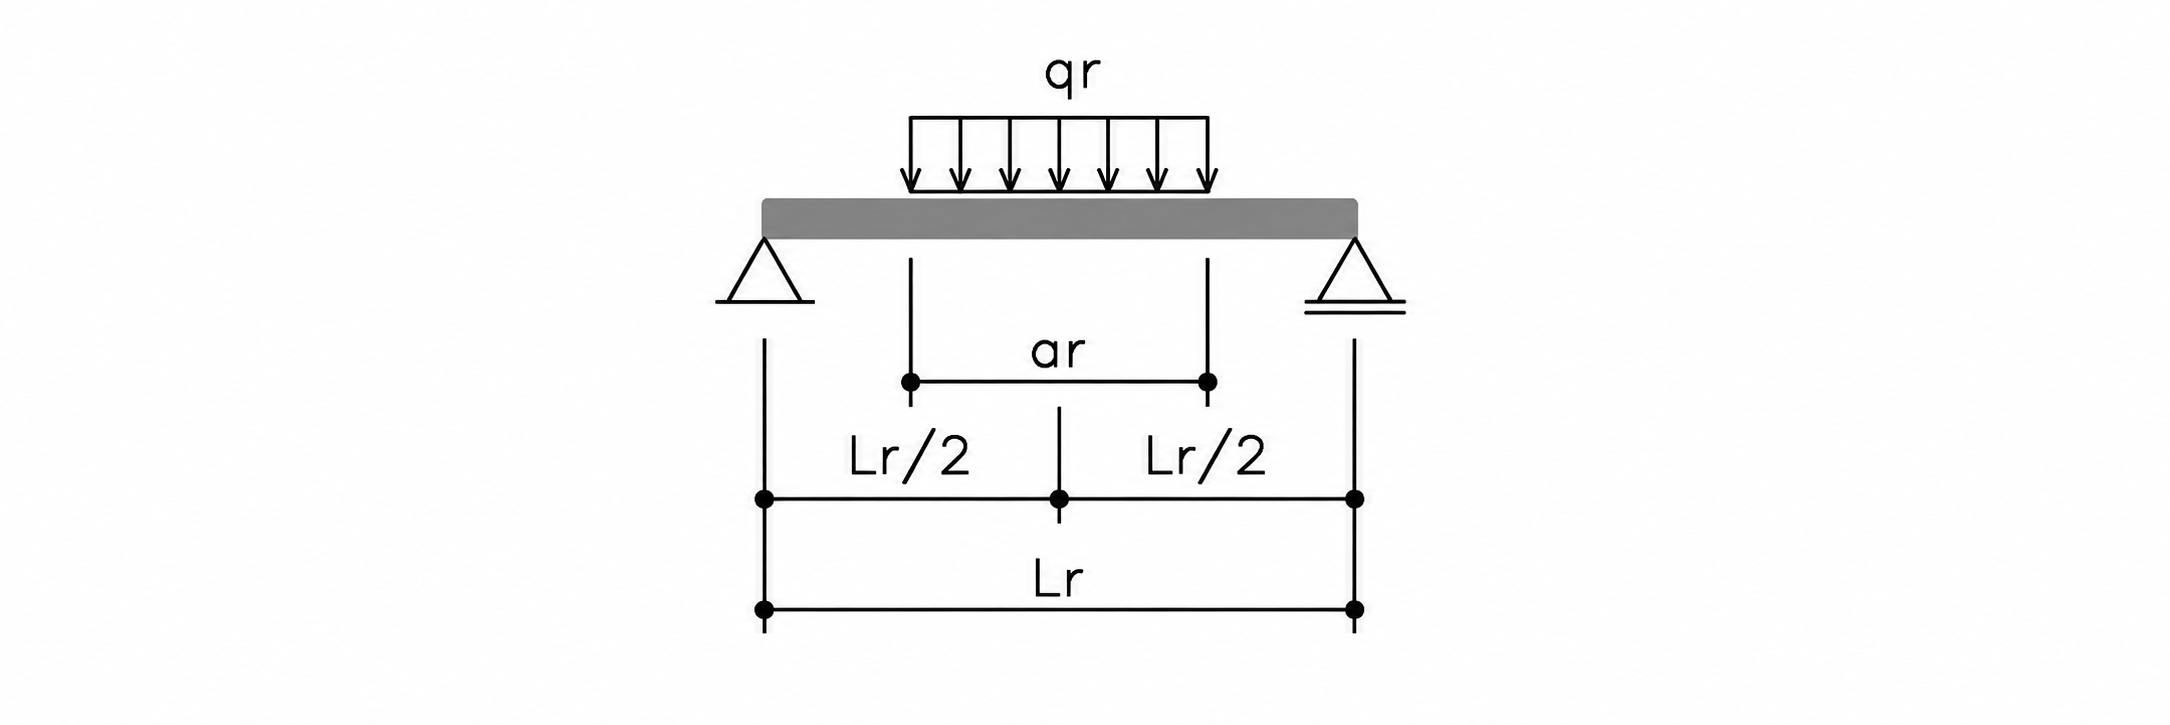
\includegraphics[trim=680bp 65bp 740bp 35bp,clip,width=0.30\textwidth]{figuras/posicionamento_roda_tabuleiro.png}
    \caption{Posicionamento crítico de uma roda sobre o tabuleiro \parencite{CALIL2006}.}
    \label{fig:posicao_tabuleiro}
\end{figure}

$M_{qk,tab}$ é então obtido pela Equação~\eqref{eq:mqktab}, em que $a_r$ é o comprimento efetivo de contato da roda sobre o tabuleiro e $CIV_{tab}$ é o coeficiente de impacto vertical calculado de forma análoga às Equações~\eqref{eq:civ1} e~\eqref{eq:civ2}, considerando como vão de referência o espaçamento $esp_{long}$.

\begin{equation}
M_{qk,tab} = \frac{P}{4}\,\left(esp_{long} - a_r\right)\cdot CIV_{tab}
\label{eq:mqktab}
\end{equation}

O momento de cálculo do tabuleiro, $M_{sd,tab}$, segue a mesma combinação de ações da Equação~\eqref{eq:comb}.
A verificação de flexão do tabuleiro segue o mesmo critério empregado para a longarina (Equação~\eqref{eq:verflexao}), comparando a tensão normal solicitante $\sigma_{x,d,tab} = M_{sd,tab}/W_{x,tab}$ com a resistência de cálculo à flexão do tabuleiro $f_{md,tab}$, calculada conforme a Equação~\eqref{eq:2.099}.
